\section{Timing system}
\label{sec:tim_sys}

\begin{figure}[ht]
  \begin{center}
    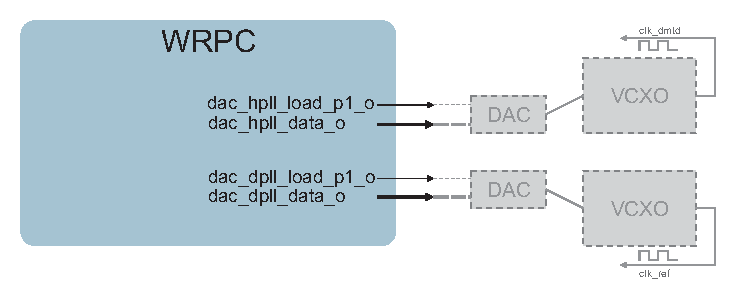
\includegraphics[width=.8\textwidth]{fig/wrpc_tsys.pdf}
  \end{center}
\end{figure}

Timing system outputs are mandatory part of WRPC PLLs that discipline local
oscillators.

\begin{center}
  \begin{tabular}{|l|l|p{11cm}|}
    \hline {\bf name} & {\bf size} & {\bf description} \\
    \hline
    \emph{dac\_hpll\_load\_p1\_o} & 1 & validates DAC value on data port \\
    \emph{dac\_hpll\_data\_o} & 16 & DAC value for tuning helper (DMTD) VCXO\\
    \hline
    \emph{dac\_dpll\_load\_p1\_o} & 1 & validates DAC value on data port \\
    \emph{dac\_dpll\_data\_o} & 16 & DAC value for tuning main (ref) VCXO\\
    \hline
  \end{tabular}
\end{center}
